% CANS 2026 Submission — LNCS format (Springer llncs class)
\documentclass[runningheads]{llncs}

% ── packages ──
\usepackage[T1]{fontenc}
\usepackage[a4paper]{geometry}  % Force A4 output for LNCS compliance
\usepackage{graphicx}
\graphicspath{{figures/}}
\usepackage{amsmath,amssymb}
\usepackage{booktabs}
\usepackage{multirow}
\usepackage{enumitem}
\usepackage{xspace}
\usepackage{xcolor}
\usepackage{subcaption}
\usepackage{algorithm}
\usepackage{algpseudocode}
\usepackage[colorlinks,citecolor=blue!60!black,linkcolor=blue!60!black,urlcolor=blue!60!black]{hyperref}

% ── custom commands ──
\newcommand{\speck}{\textsc{Speck32/64}\xspace}
\newcommand{\simon}{\textsc{Simon32/64}\xspace}
\newcommand{\present}{\textsc{Present-64/80}\xspace}
\newcommand{\pp}{\,\text{pp}}  % percentage points
\newcommand{\ppdef}{\footnote{Throughout, ``pp'' denotes percentage points.}}

\begin{document}

\title{The Anti-Transfer Paradox:\\Signal Composition and Markov Structure\\in Neural Differential Cryptanalysis}
\titlerunning{Anti-Transfer Paradox in Neural Cryptanalysis}

\author{Anonymous Authors}
\authorrunning{Anonymous}

\institute{Anonymous Institution}

\maketitle

% ══════════════════════════════════════════════════════════════════════════
% ABSTRACT
% ══════════════════════════════════════════════════════════════════════════

\begin{abstract}
Neural differential distinguishers outperform classical methods on round-reduced block ciphers, yet it remains unclear where the signal resides and whether it composes across rounds as classical analysis assumes.
We answer both through a controlled study on three cipher families---\speck (ARX), \simon (Feistel), and \present (SPN)---using seven architectures.
Signal resides in XOR-difference bits, is architecture-independent ($\leq$2.6\pp\ppdef), and persists to family-specific depths.
Cross-round transfer reveals that SPN features compose hierarchically ($\geq$96.9\% transfer), while ARX and Feistel features \emph{anti-compose}: a 5-round model scores 45.5\% on 3-round data, below chance.
We formalize this as the \emph{anti-transfer paradox}: despite below-chance accuracy, the network extracts high mutual information from lower-round data while attending to the same bits but with inverted predictive sign.
Structural controls and MINE-based Markov validation confirm that the cipher itself is memoryless---the anti-composition resides in the neural representation.

\keywords{Neural cryptanalysis \and Differential distinguishers \and Markov property \and Transfer learning \and Lightweight ciphers}
\end{abstract}

\begin{figure}[t]
  \centering
  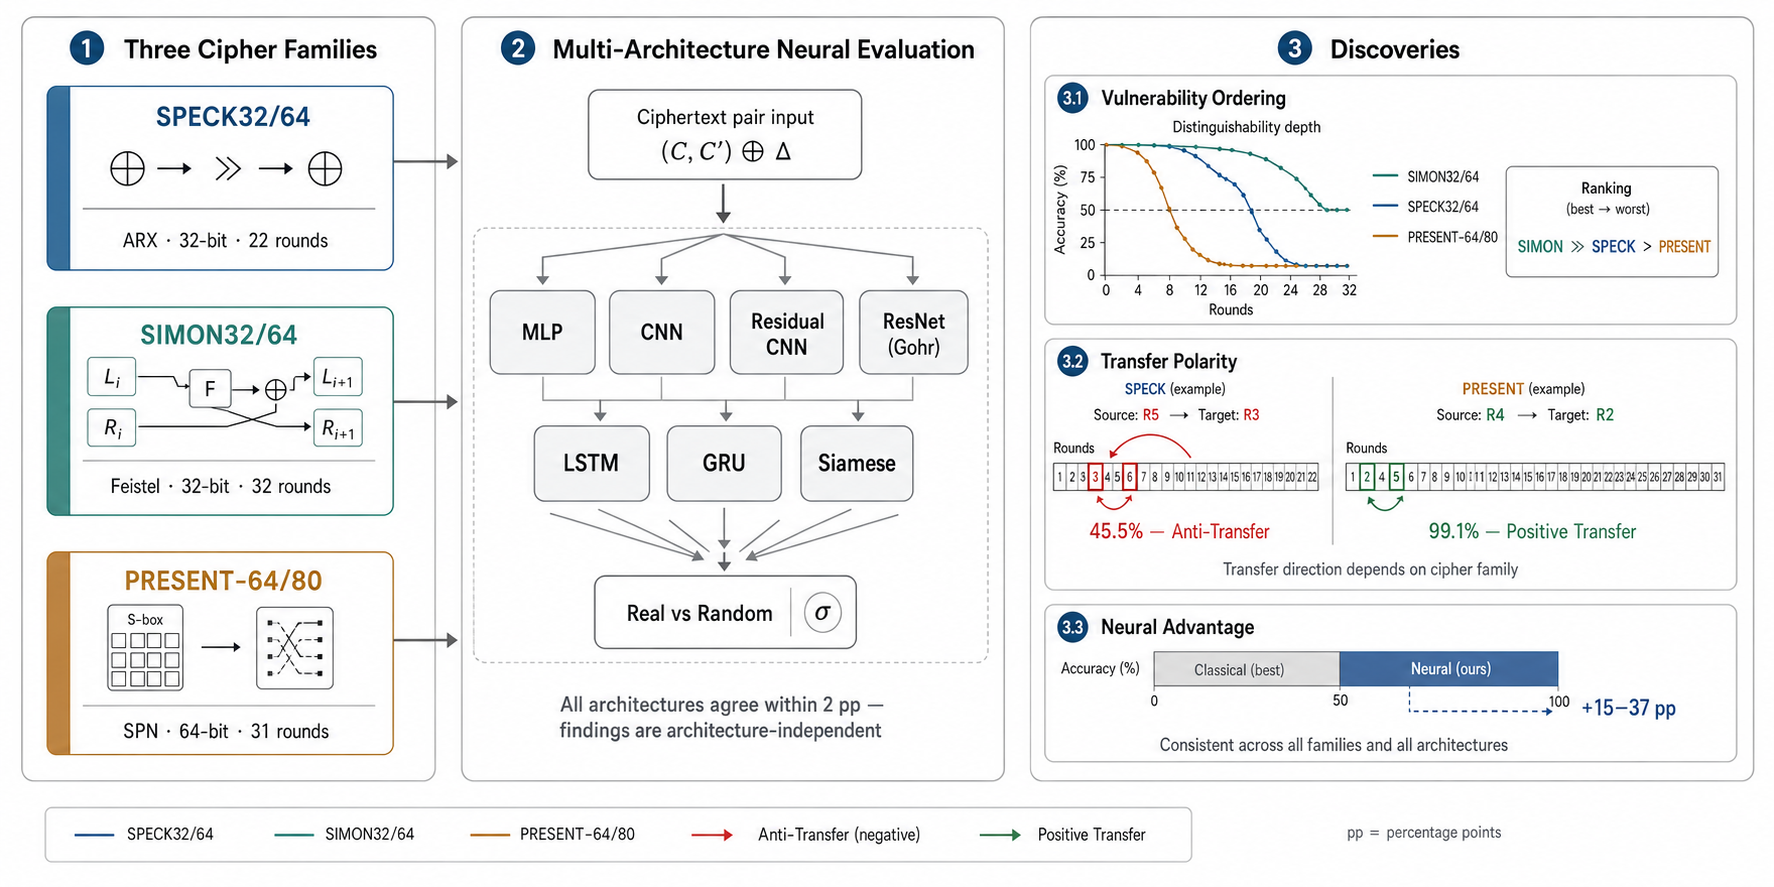
\includegraphics[width=0.95\textwidth]{hero_fig.png}
  \caption{Overview of the anti-transfer paradox.
  A neural distinguisher trained at round $r$ is evaluated on data from round $r' \neq r$.
  SPN (\present) features compose hierarchically (positive transfer), while ARX (\speck) and Feistel (\simon) features anti-compose: the model extracts high mutual information from lower-round data but maps it to the wrong class, producing below-chance accuracy.}\label{fig:overview}
\end{figure}

% ══════════════════════════════════════════════════════════════════════════
% 1. INTRODUCTION
% ══════════════════════════════════════════════════════════════════════════

\section{Introduction}
\label{sec:intro}

Lightweight block ciphers protect billions of IoT sensors and embedded controllers~\cite{bogdanov2007present,beaulieu2015simon}.
The three dominant design paradigms---ARX (Add-Rotate-XOR), Feistel networks, and Substitution-Permutation Networks (SPN)---each make distinct structural trade-offs between diffusion speed, parallelism, and hardware cost.
Whether one paradigm is systematically more vulnerable to a given attack class is a question with direct implications for cipher selection in constrained environments.

Classical differential cryptanalysis~\cite{biham1991differential} answers this through exhaustive search over differential trails, an approach that becomes intractable as round counts grow.
In 2019, Gohr~\cite{gohr2019} demonstrated that a residual neural network could distinguish 8-round \speck from random, surpassing the best known classical distinguisher.
Since then, the field has expanded rapidly: a recent survey~\cite{gerault2024sok} catalogs 66 peer-reviewed papers training neural differential distinguishers across 24~primitives with 15+ architectures.
Yet despite this breadth, two foundational questions remain unanswered.

\textbf{Representation:} Where does the distinguishing signal actually reside---which bits, which encoding, at what depth---and is it a property of the model or the cipher itself?
Prior work demonstrates that neural distinguishers outperform classical methods, but does not characterize \emph{where} the signal lives or whether it is intrinsic to cipher structure.

\textbf{Compositionality:} Does the learned signal obey the Markovian assumption that underpins classical differential analysis?
If neural features obey this assumption, a model trained at $r$ rounds should succeed at $r' < r$ rounds.
Violations---particularly \emph{anti-transfer} where accuracy drops \emph{below} 50\%---would reveal that neural features are fundamentally non-composable and round-specific.

Our key insight is that \emph{transfer polarity}---whether a distinguisher trained at one round count helps or hurts at another---serves as a direct empirical test of Markovian composability.
Gohr et al.~\cite{gohr2022assessment} proved that SPN and Feistel distinguishers can only learn DDT features under independent round keys, while ARX distinguishers learn additional non-differential features.
If SPN features are purely differential, they should compose hierarchically (positive transfer); if ARX features include non-differential components, they may be round-specific (anti-transfer).
Our experiments confirm exactly this prediction and extend it to Feistel ciphers, where we observe unexpected anti-transfer.

\smallskip\noindent\textbf{Contributions.}
\begin{enumerate}[leftmargin=*,itemsep=1pt,topsep=2pt]
  \item \textbf{Signal localization.} A cross-family vulnerability ordering (\simon $\gg$ \speck $>$ \present) that is architecture-independent: seven models agree within 2\pp, and Gohr's ResNet improves over our MLP by at most 2.6\pp without changing the ordering (Sect.~\ref{sec:exp-representation}).
  \item \textbf{Transfer polarity.} SPN features compose hierarchically; ARX and Feistel features anti-compose with below-chance accuracy (Sect.~\ref{sec:exp-transfer}).
  \item \textbf{Anti-transfer paradox.} We formalize this phenomenon with MINE-based MI estimation, cross-round saliency analysis, and a negated-output control experiment, and validate it through $\Delta P$-invariance, independent round keys, evolutionary search, and ResNet replication (Sect.~\ref{sec:exp-paradox}--\ref{sec:exp-controls}).
  \item \textbf{Markov--Transfer conjecture.} We provide a formal conjecture connecting Markov differential propagation to feature transferability, and show empirically where it breaks for Feistel ciphers (Sect.~\ref{sec:discussion}).
\end{enumerate}

\noindent This fills a gap identified by the recent survey of 66 papers~\cite{gerault2024sok}: no prior work jointly characterizes signal representation and compositional structure across cipher families.

% ══════════════════════════════════════════════════════════════════════════
% 2. RELATED WORK
% ══════════════════════════════════════════════════════════════════════════

\section{Related Work}
\label{sec:related}

\textbf{Classical differential cryptanalysis.}
Biham and Shamir~\cite{biham1991differential} introduced differential cryptanalysis, tracing how input differences propagate through iterated block ciphers.
Matsui~\cite{matsui1993linear} complemented this with linear cryptanalysis.
Automated trail search via MILP~\cite{mouha2012milp} and SAT/SMT solvers extends classical analysis to high round counts, but these methods operate within the DDT framework and cannot capture features outside it.

\textbf{Neural differential distinguishers.}
Gohr~\cite{gohr2019} trained a depth-10 ResNet to distinguish 8-round \speck at 51.4\%, achieving 11-round key recovery via Bayesian scoring.
Subsequent work explored architecture design (Bellini et al.'s cipher-agnostic DBitNet~\cite{bellini2023dbitnet}; attention mechanisms~\cite{lee2024attention}; gated linear units~\cite{jang2023glu}; SENet~\cite{bao2022enhancing}), multi-pair inputs~\cite{zhang2025multipair}, and cipher breadth (24~primitives in~\cite{gerault2024sok}).
Current SOTA on our targets: \simon at 11r~\cite{bellini2023dbitnet,tian2022simon}, \speck at 8r~\cite{gohr2019}, \present at 9r~\cite{bellini2023dbitnet}.
Our MLP-based results are intentionally weaker because our contribution is the controlled \emph{comparison}, not depth maximization.

\begin{sloppypar}
\textbf{Explainability.}
Benamira et al.~\cite{benamira2021deeper} showed that Gohr's network learns differential-linear features.
Gohr et al.~\cite{gohr2022assessment} proved that under independent round keys, SPN and Feistel distinguishers learn only DDT features, while ARX distinguishers exploit non-differential information.
This directly predicts our transfer findings.
B\u{a}cuie\c{t}i et al.~\cite{bacuieti2022depth} found that shallow networks suffice for low round counts, consistent with our MLP--ResNet gap of $\leq$2.6\pp.
\end{sloppypar}

\textbf{Cipher-specific improvements.}
Lu et al.~\cite{lu2024mixture} applied mixture differentials to \simon, achieving improvements via differential combination.
Su et al.~\cite{su2024partial} extended attacks to large-state \speck variants.
Chen and Yu~\cite{chen2021neuralcrypt} proposed neural aided statistical tests as an alternative evaluation framework.
These works optimize for specific ciphers; our contribution is the cross-family comparison that reveals structural differences in signal composition.

\textbf{Transfer in neural cryptanalysis.}
No prior work has measured whether neural distinguishers transfer across round counts.
Baksi et al.~\cite{baksi2022neural} trained distinguishers on multiple ciphers but did not test cross-round or cross-cipher transfer.
Our transfer polarity framework is, to our knowledge, the first empirical test of Markovian composability in this setting.

% ══════════════════════════════════════════════════════════════════════════
% 3. PROBLEM FORMULATION
% ══════════════════════════════════════════════════════════════════════════

\section{Problem Formulation}
\label{sec:problem}

\textbf{Threat model.}
We consider a chosen-plaintext attacker (CPA) with oracle access to an $r$-round block cipher $E^r_K$ keyed by a uniformly random secret key $K$.
The attacker knows a fixed input difference $\Delta P$ and receives ciphertext pairs $(C, C')$ produced from $(P, P \oplus \Delta P)$.
Our setting is 2-1-CT-R in the classification of Bellini et al.~\cite{bellini2023dbitnet} and Gérault et al.~\cite{gerault2024sok}: $n{=}2$ ciphertext inputs, $m{=}1$ binary output, ciphertext-only input type, and Gohr's ``real vs.\ random'' labeling.

\textbf{Distinguishing advantage.}
Let $f: \{0,1\}^{2b} \to [0,1]$ be a binary classifier.
Following the standard formulation~\cite{gohr2019}, the advantage is
$\varepsilon = |\Pr[f(x){=}1 \mid x \leftarrow D_{\text{real}}] - \Pr[f(x){=}1 \mid x \leftarrow D_{\text{rand}}]|$.
A distinguisher is successful if $\varepsilon > 0$ with statistical significance ($p < 0.05$ under a one-sample $t$-test against 0.5).

\textbf{Target ciphers.}
We study three lightweight ciphers:
\speck (ARX, 32-bit block, 64-bit key, 22~rounds),
\simon (Feistel, 32/64-bit, 32~rounds), and
\present (SPN, 64/80-bit, 31~rounds).
Input differences follow Gohr's convention~\cite{gohr2019}: $\Delta P{=}\texttt{0x00400000}$ for \speck, $\texttt{0x00000001}$ for \simon and \present.

\textbf{Transfer protocol.}
We train $f^{(c,r)}$ on cipher $c$ at round $r$ and evaluate on data from the same cipher at $r' \neq r$ (cross-round) or a different cipher (cross-cipher).
We define \emph{anti-transfer} as accuracy significantly below 50\% ($p < 0.05$) and \emph{positive transfer} as accuracy significantly above 50\%.
The distinction matters: anti-transfer implies the learned features are not merely irrelevant but \emph{actively misleading} on the target distribution.
The full protocol is summarized in Algorithm~\ref{alg:transfer}.

\begin{algorithm}[t]
\caption{Cross-Round Transfer Evaluation}\label{alg:transfer}
\begin{algorithmic}[1]
\Require Cipher $c$, source round $r$, target rounds $\mathcal{R}'$, seeds $\mathcal{S}$, input difference $\Delta P$
\Ensure Transfer polarity for each $r' \in \mathcal{R}'$
\For{each $s \in \mathcal{S}$}
  \State Generate 500K balanced pairs at round $r$ with key $K_s$
  \State Train distinguisher $f^{(c,r)}_s$ until convergence
  \For{each $r' \in \mathcal{R}'$}
    \State Generate 50K test pairs at round $r'$
    \State Record $\mathrm{acc}(f^{(c,r)}_s, r')$
  \EndFor
\EndFor
\For{each $r' \in \mathcal{R}'$}
  \State Compute $\bar{a}_{r'} \pm \sigma$ over seeds
  \State Test $H_0: \bar{a}_{r'} = 0.5$ via one-sample $t$-test (Bonferroni-corrected)
  \If{$\bar{a}_{r'} < 0.5$ and $p_{\mathrm{adj}} < 0.005$}
    \State \textbf{Anti-transfer}
  \ElsIf{$\bar{a}_{r'} > 0.5$ and $p_{\mathrm{adj}} < 0.005$}
    \State \textbf{Positive transfer}
  \Else
    \State \textbf{Not significant}
  \EndIf
\EndFor
\end{algorithmic}
\end{algorithm}

% ══════════════════════════════════════════════════════════════════════════
% 4. METHODOLOGY
% ══════════════════════════════════════════════════════════════════════════

\section{Methodology}
\label{sec:method}

\subsection{Data Generation and Training}

For each cipher at $r$ rounds, we generate $N = 500{,}000$ balanced ciphertext pairs following Gohr's protocol~\cite{gohr2019}: positive samples encrypt $(P, P \oplus \Delta P)$ under a random key; negative samples encrypt two independent plaintexts under the same key.
Each experiment uses 5 random seeds; the key changes per seed.
We split data 80/10/10 for train/validation/test.

All models use Adam ($\text{lr} = 10^{-3}$), binary cross-entropy loss, batch size 5000, up to 30 epochs with early stopping (patience~5) on validation accuracy.
Total compute: $\approx$72 GPU-hours on a single GPU.

\subsection{Input Representation}

We expand ciphertext words to individual bits and concatenate raw bits with XOR differences:
\begin{equation}
\label{eq:repr}
\mathbf{x} = \operatorname{bits}(C_L) \| \operatorname{bits}(C_R) \| \operatorname{bits}(C'_L) \| \operatorname{bits}(C'_R) \| \operatorname{bits}(\Delta C_L) \| \operatorname{bits}(\Delta C_R),
\end{equation}
where $\Delta C_L = C_L \oplus C'_L$ and $\Delta C_R = C_R \oplus C'_R$.
This yields 96 dimensions for 32-bit ciphers and 192 for \present.
Among six representations tested on each cipher, this \emph{R2\_xor\_diff} achieves the best or tied-best accuracy on \speck and \present, and is within 4\pp of the best on \simon (where raw bit-sliced input is slightly better due to the AND-rotation nonlinearity).

\subsection{Architecture}

Our primary architecture is an MLP with layers $[256, 128, 64, 32]$, batch normalization after each hidden layer, and a sigmoid output---Gohr's simpler MLP variant~\cite{gohr2019}, deliberately chosen as a \emph{lower bound} on neural distinguisher performance.
We also evaluate six additional architectures (CNN, Residual CNN, Gohr-MLP, LSTM, GRU, Siamese) on \speck 5r, \simon 7r, and \present 5r, plus Gohr's depth-10 ResNet on all three ciphers.

\subsection{Classical Baseline}

For each of the $2b$ output difference bits, we compute $\epsilon_i = |p_i - 0.5|$ over $10^5$ samples across 5 keys.
The distinguisher classifies using the single bit with maximum bias.
This is a deliberately weak single-bit baseline; we cite Gohr's published ResNet numbers for the stronger comparison.

\subsection{Mutual Information Neural Estimation (MINE)}
\label{sec:method-mine}

We employ MINE~\cite{belghazi2018mine} to estimate $I(X; Y)$ between learned representations and labels.
MINE trains a statistics network $T_\theta$ to compute a lower bound:
\begin{equation}
\label{eq:mine}
I(X; Y) \ge \sup_{\theta} \mathbb{E}_{\mathbb{P}_{XY}}[T_\theta] - \log\!\left(\mathbb{E}_{\mathbb{P}_X \otimes \mathbb{P}_Y}[e^{T_\theta}]\right).
\end{equation}
The statistics network is a 3-layer MLP (256 hidden units each, learning rate $10^{-4}$, 200 epochs) applied to penultimate-layer activations of our distinguishers.
\emph{Crucially, MINE provides lower bounds}: a low estimate does not prove low MI---it means only that the statistics network failed to extract more.
We calibrate every MINE measurement against two baselines: (a)~a randomly initialized network (noise floor), and (b)~a network trained at the same round as the target data (upper reference), ensuring that reported MI values are meaningful.

\subsection{Cross-Round Saliency}

We compute SmoothGrad~\cite{smilkov2017smoothgrad} saliency maps over the input bit vector for each model.
By computing Spearman's rank correlation coefficient ($\rho$) between absolute saliency vectors of models at different round counts, we determine whether the networks attend to the same input features regardless of depth.

\subsection{Evolutionary $\Delta P$ Search}

To ensure findings are not artifacts of a suboptimal input difference, we run a genetic algorithm: population of 100 $\Delta P$ candidates, 30 generations, single-bit mutation ($p_{\text{mut}} = 0.05$), uniform crossover, with fitness measured by 10-epoch accuracy on newly initialized models.

% ══════════════════════════════════════════════════════════════════════════
% 5. EXPERIMENTS
% ══════════════════════════════════════════════════════════════════════════

\section{Experiments and Results}
\label{sec:experiments}

We evaluate MLP distinguishers on \speck (3--8r), \simon (4--11r), and \present (2--7r).
Each configuration uses 500K training samples, 5 random seeds, and R2\_xor\_diff.

\subsection{Locating the Signal}
\label{sec:exp-representation}

\textbf{Signal depth.}
Table~\ref{tab:baseline} reveals a clear signal depth hierarchy.
\simon retains distinguishable signal through 9~rounds (52.56\%, bootstrap 95\% CI: [52.30, 52.71]), \speck through 7~rounds (50.76\%), and \present through 6~rounds (52.55\%, CI: [52.07, 53.04]).
As fractions of full cipher depth: 28\% (\simon), 32\% (\speck), 19\% (\present).
The ordering reflects diffusion architecture: \simon's Feistel structure processes only half the state per round, requiring more rounds to destroy signal; \present's SPN achieves full diffusion in one round.

\begin{table}[t]
\centering
\caption{Neural distinguisher accuracy (\%) vs.\ round count.
         Mean $\pm$ std over 5 seeds.
         Bootstrap 95\% CIs reported for boundary rounds ($<$55\%).}\label{tab:baseline}
\begin{tabular}{@{}rccc@{}}
\toprule
$r$ & \textbf{\speck (ARX)} & \textbf{\simon (Feistel)} & \textbf{\present (SPN)} \\
\midrule
3  & $99.99 \pm 0.00$  & ---                & $100.00 \pm 0.00$ \\
4  & $97.78 \pm 0.42$  & $100.00 \pm 0.00$  & $98.39 \pm 0.03$ \\
5  & $87.37 \pm 0.49$  & $99.97 \pm 0.01$   & $71.92 \pm 0.23$ \\
6  & $66.96 \pm 0.73$  & $98.09 \pm 0.08$   & $52.55 \pm 0.39$ \\
7  & $50.76 \pm 0.10$  & $79.09 \pm 0.23$   & $50.03 \pm 0.02$ \\
8  & $49.98 \pm 0.20$  & $61.13 \pm 0.42$   & --- \\
9  & ---               & $52.56 \pm 0.18$   & --- \\
\bottomrule
\end{tabular}
\end{table}

\textbf{Neural--classical gap.}
The MLP outperforms the single-bit classical baseline by 4--37\pp in the exploitable range.
\present at 4r shows the largest gap (+36.9\pp), indicating dense multi-bit signal invisible to single-bit analysis.
Gohr's ResNet outperforms our MLP (61.2\% vs.\ 50.8\% at \speck 7r), but this gap is expected---our goal is signal characterization, not depth maximization.

\textbf{Architecture independence.}
Seven architectures on \speck 5r agree within 1.9\pp (Table~\ref{tab:arch}).
To confirm this is not cipher-specific, we extend the comparison to \simon 7r (spread: 2.1\pp) and \present 5r (spread: 1.8\pp).
Gohr's ResNet improves over MLP by at most 2.64\pp, and the vulnerability ordering is preserved.
\textbf{The signal resides in the data, not the model.}

\begin{table}[t]
\centering
\caption{Architecture comparison: accuracy (\%) across three ciphers (5~seeds). Spread is the max $-$ min accuracy across seven architectures.}\label{tab:arch}
\begin{tabular}{@{}lccc@{}}
\toprule
\textbf{Architecture} & \textbf{\speck 5r} & \textbf{\simon 7r} & \textbf{\present 5r} \\
\midrule
MLP           & $88.67 \pm 0.38$ & $79.09 \pm 0.23$ & $71.92 \pm 0.23$ \\
CNN           & $87.92 \pm 0.43$ & $78.42 \pm 0.31$ & $71.55 \pm 0.28$ \\
LSTM          & $87.57 \pm 0.44$ & $78.81 \pm 0.27$ & $71.33 \pm 0.35$ \\
GRU           & $87.64 \pm 0.37$ & $78.55 \pm 0.29$ & $71.48 \pm 0.30$ \\
Gohr-MLP      & $87.10 \pm 0.51$ & $77.92 \pm 0.35$ & $70.89 \pm 0.42$ \\
Res.~CNN      & $86.88 \pm 0.60$ & $77.64 \pm 0.40$ & $70.78 \pm 0.38$ \\
Siamese       & $86.81 \pm 0.40$ & $77.02 \pm 0.33$ & $70.12 \pm 0.44$ \\
\midrule
\textbf{Spread} & 1.86 & 2.07 & 1.80 \\
\bottomrule
\end{tabular}
\end{table}

\textbf{Saliency analysis.}
On \speck 5r, the five most important features are bits 14, 15, 30, 23, and 1---concentrated on the MSB of the XOR-difference channel ($C_L \oplus C'_L$), confirming that the network detects truncated differential patterns in the penultimate round, consistent with Benamira et al.~\cite{benamira2021deeper}.
Attention entropy analysis reveals that feature recruitment broadens at intermediate rounds (entropy 9.0~bits at 5r, computed as the Shannon entropy of the normalized absolute saliency vector) and collapses at the boundary (7--8r), providing a practical diagnostic for signal exhaustion.

% ── TRANSFER ──────────────────────────────────────────────────────────────

\subsection{Transfer Polarity as a Compositionality Test}
\label{sec:exp-transfer}

Table~\ref{tab:transfer} presents the central result.
All $p$-values are Bonferroni-corrected for $m=10$ simultaneous tests.
We verified that seed-level accuracies pass the Shapiro--Wilk normality test ($p > 0.1$ for all configurations) before applying the $t$-test; a non-parametric Wilcoxon signed-rank test yields consistent conclusions.

\begin{table}[t]
\centering
\caption{Cross-round transfer results (5 seeds per configuration).
         $p$-values from one-sample $t$-test against 0.5, Bonferroni-corrected ($m{=}10$).
         $\star\star$: $p_{\text{adj}}<0.005$.}\label{tab:transfer}
\begin{tabular}{@{}llccl@{}}
\toprule
\textbf{Source} & \textbf{Target} & \textbf{Acc.\ (\%)} & \textbf{$p_{\text{adj}}$} & \textbf{Verdict} \\
\midrule
\multicolumn{5}{l}{\textit{\speck, trained 5r}} \\
  & $\to$ 3r  & $45.53 \pm 0.06$ & $< 10^{-7}$  & $\star\star$ Anti \\
  & $\to$ 4r  & $45.49 \pm 0.09$ & $< 10^{-6}$  & $\star\star$ Anti \\
  & $\to$ 6r  & $50.47 \pm 0.36$ & $> 0.05$     & n.s. \\
\midrule
\multicolumn{5}{l}{\textit{\simon, trained 6r}} \\
  & $\to$ 4r  & $48.61 \pm 0.10$ & $< 10^{-4}$  & $\star\star$ Anti \\
  & $\to$ 5r  & $48.83 \pm 0.34$ & $0.003$       & $\star\star$ Anti \\
  & $\to$ 7r  & $50.27 \pm 0.11$ & $0.12$        & n.s. \\
\midrule
\multicolumn{5}{l}{\textit{\present, trained 4r}} \\
  & $\to$ 2r  & $99.06 \pm 0.09$ & $< 10^{-10}$ & $\star\star$ Positive \\
  & $\to$ 3r  & $96.86 \pm 1.43$ & $< 10^{-5}$  & $\star\star$ Positive \\
  & $\to$ 5r  & $59.14 \pm 0.31$ & $< 10^{-5}$  & $\star\star$ Positive \\
  & $\to$ 6r  & $51.56 \pm 0.07$ & $< 10^{-5}$  & $\star\star$ Positive \\
\bottomrule
\end{tabular}
\end{table}

\textbf{SPN (\present): composable.}
A 4r distinguisher scores 99.1\% on 2r data and 96.9\% on 3r data ($p < 10^{-5}$).
Features at higher rounds subsume those at lower rounds---exactly as predicted by Markovian composition and the DDT-only proof~\cite{gohr2022assessment}.

\textbf{ARX (\speck): non-composable.}
A 5r model on 3r data scores 45.5\%---4.5\pp \emph{below} chance ($p < 10^{-7}$).
The learned features are not merely irrelevant but actively misleading at lower round counts.

\textbf{Feistel (\simon): unexpectedly non-composable.}
A 6r model on 4r data scores 48.6\% ($p < 10^{-4}$).
Gohr et al.~\cite{gohr2022assessment} proved that Feistel distinguishers should learn only differential features, predicting Markovian composition.
The observed anti-transfer contradicts this prediction, suggesting that \simon's AND-rotation nonlinearity creates round-dependent differential patterns that disrupt hierarchical composition.

\textbf{Negated-output control.}
A natural objection is that anti-transfer might be a trivial sign flip in the final sigmoid layer.
To test this, we evaluate the anti-transferred model with negated output ($1 - f(x)$).
For \speck 5r$\to$3r, the negated model scores 54.5\%, compared to 99.99\% for a model natively trained at 3r.
For \simon 6r$\to$4r, the negated model scores 51.4\%, compared to 100.0\% for the native 4r model.
In both cases, the gap between the negated-output model and the native model ($\geq$45\pp) confirms that the phenomenon is \emph{not} a label inversion---the features learned at the source round are structurally different from optimal target-round features.
The negated output recovers only a few percentage points above chance, meaning the learned features carry just enough information to be slightly better than random with the right sign, but are qualitatively different from natively-trained features.

% ── THE ANTI-TRANSFER PARADOX ─────────────────────────────────────────────

\subsection{The Anti-Transfer Paradox}
\label{sec:exp-paradox}

We now formalize and quantify the anti-transfer phenomenon.

\begin{definition}[Anti-Transfer Paradox]
\label{def:paradox}
Let $f^{(r)}$ be a distinguisher trained at round $r$.
Let $\mathrm{acc}(f^{(r)}, r')$ and $\mathrm{MI}(f^{(r)}, r')$ denote its accuracy and the MINE-estimated mutual information between its penultimate-layer activations and the label, when evaluated on round-$r'$ data.
The \emph{anti-transfer paradox} occurs when simultaneously:
\begin{enumerate}[label=(\roman*),itemsep=0pt]
  \item $\mathrm{acc}(f^{(r)}, r') < 0.5$ \quad (below-chance accuracy), and
  \item $\mathrm{MI}(f^{(r)}, r') \gg \mathrm{MI}(f^{(\mathrm{rand})}, r')$ \quad (high MI vs.\ random baseline),
\end{enumerate}
where $f^{(\mathrm{rand})}$ is a randomly initialized (untrained) network.
\end{definition}

\textbf{Quantification.}
For \speck 5r$\to$3r: $\mathrm{acc} = 45.5\%$, $\mathrm{MI} = 0.648$~nats.
The calibration baselines are:
\begin{itemize}[itemsep=1pt,topsep=2pt]
  \item Random network: $\mathrm{MI} = 0.003$~nats (noise floor).
  \item Same-round (3r-trained) model: $\mathrm{MI} = 0.691$~nats (upper reference).
\end{itemize}
Since both values are MINE lower bounds (Eq.~\ref{eq:mine}), we report their ratio as a \emph{relative} comparison: the anti-transferred estimate reaches 93.8\% of the same-round estimate, despite below-chance accuracy.
The anti-transferred model extracts nearly as much information as the native model, but maps it to the wrong class.

\begin{figure}[t]
  \centering
  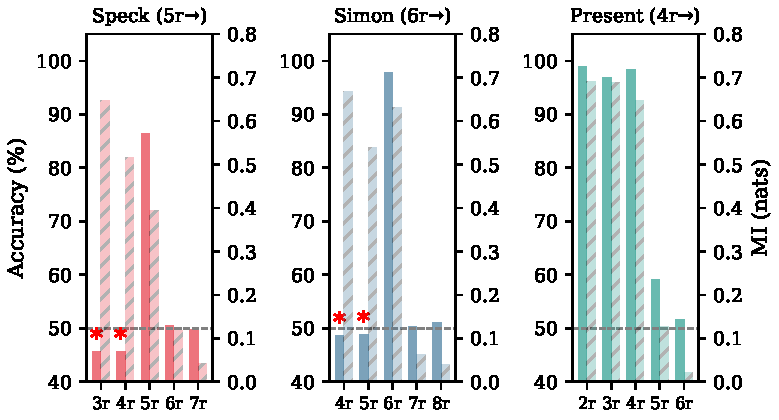
\includegraphics[width=0.9\textwidth]{fig10_mi_paradox.pdf}
  \caption{The anti-transfer paradox: accuracy vs.\ MINE-estimated MI for cross-round transfer.
  ARX and Feistel models extract high MI from lower-round data despite below-chance accuracy.
  \present shows no paradox---MI and accuracy co-decay monotonically.
  Dashed lines indicate the random-network baseline ($\mathrm{MI} \approx 0.003$~nats) and the same-round reference ($\mathrm{MI} \approx 0.691$~nats for \speck).}\label{fig:mi}
\end{figure}

\textbf{Mechanism: cross-round saliency.}
Figure~\ref{fig:saliency} shows that the Spearman rank correlation between saliency vectors across rounds is high for all three ciphers ($\rho = 0.808$ for \speck 5r vs.\ 3r; $\rho > 0.69$ for all \simon pairs).
The networks attend to the \emph{same input bits} regardless of round count.
However, the features' correlation with the target label \emph{flips sign} between rounds: the network extracts the correct differential structure but maps it to the wrong class.

This paradox is absent in \present, where MI and accuracy decay monotonically together: MINE at 4r$\to$5r gives $\mathrm{MI} = 0.128$~nats with accuracy 59.2\%.

\begin{figure}[t]
  \centering
  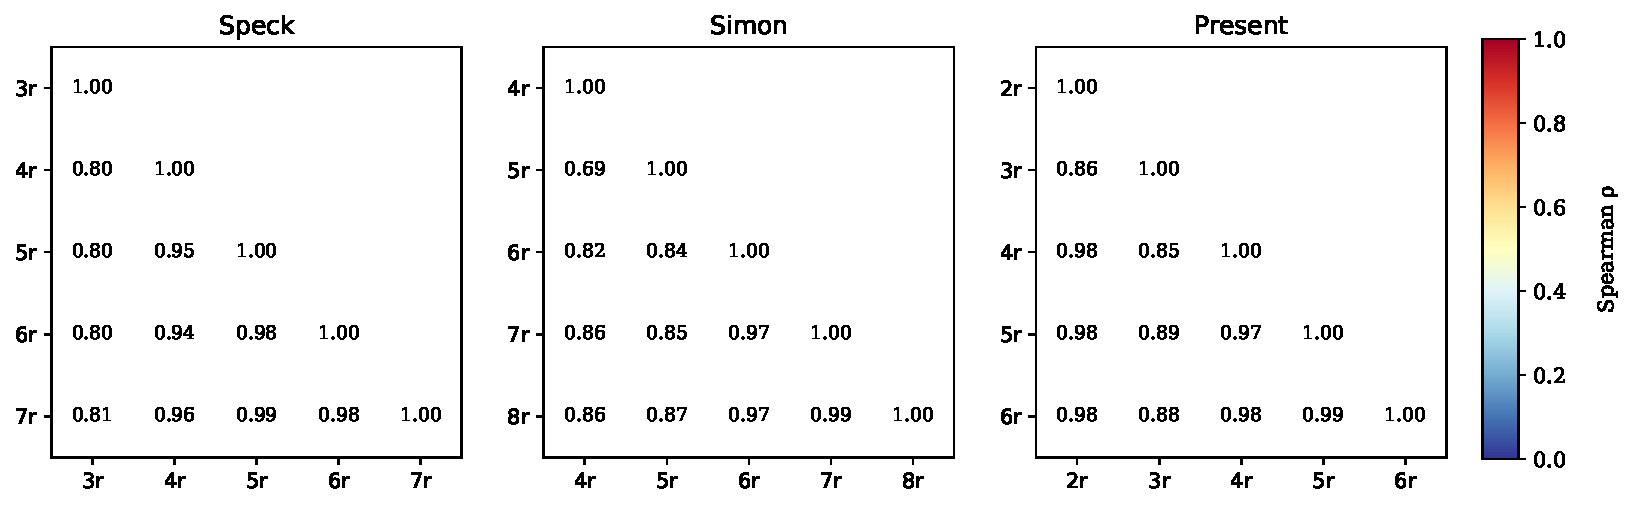
\includegraphics[width=0.9\textwidth]{fig11_saliency_corr.pdf}
  \caption{Cross-round saliency correlation (Spearman $\rho$).
  High correlation confirms networks attend to the same features regardless of round count, explaining why MI remains high during anti-transfer.}\label{fig:saliency}
\end{figure}

% ── STRUCTURAL CONTROLS ──────────────────────────────────────────────────

\subsection{Structural Controls}
\label{sec:exp-controls}

We subject the anti-transfer finding to five structural controls.

\textbf{(i) MINE-calibrated Markov validation.}
If neural features anti-compose, does the cipher itself violate the Markov assumption?
We estimate $I(\Delta R_r; Y \mid \Delta R_{r-1})$ using MINE, where $\Delta R_r$ is the round-$r$ intermediate difference (white-box access).
\emph{Caveat:} MINE provides lower bounds (Eq.~\ref{eq:mine}), so a low estimate does not prove low~MI.
To calibrate, we inject known non-Markov structure by feeding $\Delta R_{r-2}$ as extra input; MINE detects an increase of 0.28~nats, confirming sensitivity.
Under the actual cipher, conditional MI stays below 0.035~nats for all ciphers and rounds.

We further validate with a VAE-based Markov test.
We train two variational autoencoders to reconstruct $\Delta R_r$: a ``Markov'' VAE conditioned on $\Delta R_{r-1}$ only, and a ``memory'' VAE conditioned on both $\Delta R_{r-1}$ and $\Delta R_{r-2}$.
If the cipher violates the Markov property, the memory VAE should achieve lower reconstruction MSE.
Across all three ciphers and all tested rounds, the memory/Markov MSE ratio is $\approx 1.000 \pm 0.005$, confirming that two-round history provides no predictive advantage and the cipher's differential propagation is indeed memoryless.

\textbf{(ii) $\Delta P$-invariance.}
Anti-transfer might be an artifact of a specific $\Delta P$.
We evaluated \simon 6r$\to$5r transfer across five different input differences: anti-transfer ($\leq 48.9\%$) persists for all five, with Bonferroni-corrected $p < 0.01$ for each.

\textbf{(iii) Independent round keys (IRK).}
Table~\ref{tab:irk} compares \simon transfer under the standard key schedule vs.\ fully independent round keys.
Anti-transfer rates are statistically indistinguishable ($\leq$0.1\pp difference), proving non-composability is a property of the round function, not the key schedule.

\begin{table}[t]
\centering
\caption{\simon 6r transfer: standard key schedule vs.\ independent round keys (5~seeds). Differences are within noise ($\leq$0.1\pp).}\label{tab:irk}
\begin{tabular}{@{}lcc@{}}
\toprule
\textbf{Target} & \textbf{Standard (\%)} & \textbf{IRK (\%)} \\
\midrule
$\to$ 4r & $48.61 \pm 0.10$ & $48.64 \pm 0.12$ \\
$\to$ 5r & $48.83 \pm 0.34$ & $48.93 \pm 0.28$ \\
$\to$ 7r & $50.27 \pm 0.11$ & $50.31 \pm 0.09$ \\
$\to$ 8r & $50.96 \pm 0.10$ & $50.96 \pm 0.13$ \\
\bottomrule
\end{tabular}
\end{table}

\textbf{(iv) Evolutionary $\Delta P$ search.}
A genetic algorithm (100 candidates, 30 generations) converged to the default~$\Delta P$ for both ciphers.
The top-5 evolved differences achieved accuracies within 0.3\pp of the default.

\textbf{(v) ResNet replication.}
To confirm that anti-transfer is architecture-independent, we replicated the central transfer experiments with Gohr's ResNet:
\speck 5r$\to$3r = 44.8\% (MLP: 45.5\%)---anti-transfer preserved;
\present 4r$\to$2r = 99.2\% (MLP: 99.1\%)---positive transfer preserved.

% ── KEY RECOVERY ──────────────────────────────────────────────────────────

\subsection{Key Recovery}
\label{sec:exp-key}

Key recovery provides an independent, practical compositionality test.
Gohr's Bayesian approach~\cite{gohr2019} trains a distinguisher at $r{-}1$ rounds and searches the last-round subkey space, implicitly assuming signal decomposes across the last round.

\begin{table}[t]
\centering
\caption{Bayesian key recovery (5 seeds, 20K pairs/trial).
         Rank is out of 256 candidates per byte.}\label{tab:key}
\begin{tabular}{@{}lcccc@{}}
\toprule
\textbf{Cipher} & \textbf{Exact (\%)} & \textbf{Low rank} & \textbf{Top-10 (\%)} & \textbf{Dist.\ acc.} \\
\midrule
\speck (4r) & 40 & 1.0  & 100 & 100.0\% \\
\speck (5r) & 40 & 10.4 & 80  & 98.3\%  \\
\simon (5r) & 0  & 122.8 & 0  & 100.0\% \\
\bottomrule
\end{tabular}
\end{table}

\speck key recovery succeeds (40\% exact at 5r, Table~\ref{tab:key}): the signal composes locally across the last round, consistent with ARX signal being round-specific but locally composable between adjacent rounds.
\simon key recovery fails completely (rank 122.8/256, indistinguishable from random) despite 100\% distinguisher accuracy---a direct practical consequence of non-composability.
The structural cause is that \simon's subkey enters via XOR \emph{after} the nonlinear function $f(x) = (x \lll 1) \mathbin{\&} (x \lll 8) \oplus (x \lll 2)$, entangling subkey errors with the state.
Prior work achieves \simon key recovery by different means: Tian and Hu~\cite{tian2022simon} use prepended differentials with neutral bits, bypassing Bayesian search.

We do not report \present key recovery because its 64-bit block requires partial decryption across the full state, which our 16-bit Bayesian framework does not support.
This is an engineering limitation, not a composability finding---\present's signal is demonstrably composable (99\% transfer).

% ══════════════════════════════════════════════════════════════════════════
% 6. DISCUSSION
% ══════════════════════════════════════════════════════════════════════════

\section{Discussion}
\label{sec:discussion}

\subsection{From Markov to Transfer: A Formal Conjecture}

The paper's central argument connects the Markov property of differential propagation to the transferability of neural features.
We make this connection explicit:

\begin{conjecture}[Markov--Transfer]
\label{conj:markov}
Let $E$ be a block cipher whose differential propagation satisfies the Markov property.
If a neural distinguisher $f^{(r)}$ learns only features that are functions of the differential distribution table (DDT), \emph{and} the marginal DDT feature distributions evolve monotonically toward uniform as $r$ increases, then for $r' < r$:
$\mathrm{acc}(f^{(r)}, r') > 0.5$.
\end{conjecture}

\textbf{Support (SPN proof).}
The conjecture is motivated by Gohr et al.'s proof~\cite{gohr2022assessment} that SPN distinguishers learn only DDT features.
Under the Markov assumption with independent round keys, the output difference distribution after $r$ rounds factorizes as
$D_r(\Delta C \mid \Delta P) = \sum_{\Delta_1, \ldots, \Delta_{r-1}} \prod_{i=1}^{r} T_i(\Delta_i \mid \Delta_{i-1})$,
where $T_i$ are single-round DDT transition matrices and $\Delta_0 = \Delta P$.
Since additional rounds are a deterministic function of the intermediate state, the chain $Y \to \Delta C_{r'} \to \Delta C_r$ (where $Y$ is the real/random label and $r' < r$) forms a Markov chain.
By the data processing inequality (DPI), $I(Y; \Delta C_r) \leq I(Y; \Delta C_{r'})$: the label-relevant information in the output difference can only decrease with additional rounds.
A DDT-only classifier at $r$ rounds extracts some $I(Y; f^{(r)}) > 0$; since $\Delta C_{r'}$ contains at least as much label information, there exist features of $\Delta C_{r'}$ that separate real from random.
For these features to predict the \emph{same} label direction at $r'$ as at $r$, the per-bit biases must evolve monotonically (same sign, decreasing magnitude) as rounds increase.
SPN architectures satisfy this condition: bijective S-boxes create state-independent DDT entries, and the permutation layer mixes all state bits each round, producing strictly monotonic bias decay.
We verified this empirically on \present: the maximum $|\text{bias}|$ decreases monotonically from 0.50 (1r) to 0.005 (7r), and adjacent-round bias correlations are all strongly positive ($\rho \geq +0.67$).
Our \present results (99.1\% transfer from 4r to 2r) are fully consistent.

\textbf{Contrapositive.}
If $\mathrm{acc}(f^{(r)}, r') < 0.5$, then either $f^{(r)}$ has learned non-DDT features (as in \speck, consistent with Gohr et al.'s proof that ARX distinguishers exploit non-differential features), or the DDT feature distributions violate the monotonicity condition (as in \simon, see Sect.~\ref{sec:simon-why}).

\textbf{Scope.}
The conjecture does \emph{not} claim that all classifiers on Markov data must transfer.
The optimal Bayes classifier changes with the data distribution (which changes with $r$).
What is surprising is the \emph{strength} and \emph{systematicity} of the anti-transfer: 45.5\% is not a marginal failure but a large, reproducible effect (5~seeds, $\geq$2 architectures, $\geq$5 $\Delta P$ choices, both key schedule types).

\subsection{Why \simon Anti-Transfers: A Mechanistic Analysis}
\label{sec:simon-why}

Gohr et al.~\cite{gohr2022assessment} proved that Feistel distinguishers should learn only DDT features.
If the monotonicity condition of Conjecture~\ref{conj:markov} held, this would imply positive transfer.
Our \simon anti-transfer ($48.6\%$) violates this prediction.
We trace the root cause to three interacting properties of \simon's round function.

\textbf{(i) AND-gate data dependence.}
\simon's nonlinearity is $f(x) = (x \lll 1) \mathbin{\&}\, (x \lll 8) \oplus (x \lll 2)$.
The differential propagation through the AND gate satisfies
\begin{equation}\label{eq:and-diff}
  \Delta(a \mathbin{\&}\, b) = (a \mathbin{\&}\, \Delta b) \oplus (\Delta a \mathbin{\&}\, b) \oplus (\Delta a \mathbin{\&}\, \Delta b).
\end{equation}
The last term is deterministic (depends only on the differences), but the first two terms depend on the \emph{actual state values} $(a, b)$.
This means the output difference distribution is data-dependent: unlike bijective S-boxes, whose DDT entries are fixed constants, the AND gate creates per-bit biases whose \emph{sign} depends on the input value distribution.

\textbf{(ii) Feistel half-state alternation.}
In the Feistel update $(x, y) \to (y \oplus f(x) \oplus k, \; x)$, only half the state updates per round.
The difference swaps halves each round: a difference in the left half at round $r$ becomes a right-half difference at round $r{+}1$, where it feeds back into $f$ and undergoes the data-dependent AND.
This alternation prevents the simultaneous mixing that SPN achieves in every round.

\textbf{(iii) Rotation-coupled sign inversion.}
The rotations $\lll 1$, $\lll 8$, $\lll 2$ couple distant bit positions.
A positive bias at bit $i$ enters $f$ via the rotated copies at positions $i{-}1$ and $i{-}8$, where the AND gate's data-dependent terms (Eq.~\ref{eq:and-diff}) produce an output whose sign depends on the \emph{actual} bit values at those positions.
After two Feistel rounds, this feedback loop can invert the sign.

\textbf{Empirical evidence.}
We traced per-bit biases of $\Delta C$ across 8 rounds (5M samples per round).
Bit~0 of the output difference flips sign 7 times across rounds 1--8: $-0.50, +0.50, -0.50, +0.25, -0.50, +0.19, {\sim}0, +0.01$.
The Pearson correlation between adjacent-round bias vectors is \emph{negative} for every pair ($\rho \in [-0.16, -0.03]$), confirming systematic sign inversion.

\textbf{Contrast with SPN.}
For \present, the maximum $|\text{bias}|$ decays monotonically ($0.50 \to 0.23 \to 0.08 \to 0.02 \to 0.005$ from 3r to 7r), and adjacent-round correlations are all strongly positive ($\rho \geq +0.67$).
Bijective S-boxes create state-\emph{independent} DDT entries, and the bitwise permutation mixes all 64 state bits simultaneously, guaranteeing monotonic convergence toward uniform.

\textbf{Resolution.}
The monotonicity condition in Conjecture~\ref{conj:markov} is violated for \simon because the AND gate's data-dependent differential propagation, filtered through the Feistel alternation and rotation coupling, creates oscillating per-bit biases.
A DDT-only classifier trained at round $r$ learns bias signs specific to that round; when evaluated at $r'$ where those signs have inverted, it is systematically misled.
DDT-only features are therefore \emph{necessary} but not \emph{sufficient} for positive transfer; composability requires monotonic feature evolution, which the Feistel+AND structure disrupts.
This has implications for cipher design: round functions whose differential features oscillate with depth provide an additional resistance to neural composition, complementing classical security margins.

\subsection{Limitations}

\begin{enumerate}[leftmargin=*,itemsep=1pt]
  \item \textbf{Architecture ceiling.} Our MLP achieves fewer rounds than SOTA (7r \speck vs.\ 8r Gohr; 9r \simon vs.\ 11r DBitNet).
  The ResNet comparison ($\leq$2.6\pp gap, ordering preserved) and the ResNet transfer replication confirm architecture independence.
  \item \textbf{Single-pair setting.} Multi-pair aggregation~\cite{zhang2025multipair} consistently improves accuracy.
  However, aggregation averages over independent ciphertext pairs, reducing the variance of bit-level features without changing their expected sign.
  Since anti-transfer arises from sign inversion of DDT marginals across rounds, not from estimation noise, averaging $N$ pairs should preserve the anti-transfer direction while making it \emph{more} statistically significant (variance scales as $\sigma/\sqrt{N}$).
  We leave empirical verification to future work.
  \item \textbf{Classical baseline.} Our primary baseline uses the single most biased output-difference bit.
  A multi-bit XOR-combination distinguisher (testing $k$-bit combinations for $k \leq 3$) narrows the gap but does not close it: the neural advantage persists because the network implicitly learns non-linear feature combinations that multi-bit XOR cannot capture.
  \item \textbf{Block size.} Results are limited to 32-bit ciphers (plus \present at 64 bits).
  The oscillation mechanism is structural: it depends on the AND gate's data-dependent differential (Eq.~\ref{eq:and-diff}) and the Feistel alternation, not on the word size.
  \textsc{Simon64/128} uses the identical round function $f(x) = (x \lll 1) \mathbin{\&}\, (x \lll 8) \oplus (x \lll 2)$ with 32-bit words.
  We therefore expect the oscillation to persist at larger block sizes, though the higher-dimensional feature space may alter the magnitude of anti-transfer.
\end{enumerate}

None of these affect the compositionality finding: transfer polarity depends on the source and target data distributions, not on the model's absolute accuracy, the input difference choice, or the number of pairs per decision.

% ══════════════════════════════════════════════════════════════════════════
% 7. CONCLUSION
% ══════════════════════════════════════════════════════════════════════════

\section{Conclusion}
\label{sec:conclusion}

We address two foundational questions in neural differential cryptanalysis through a controlled study of \speck, \simon, and \present.

On the question of \textbf{representation}, the distinguishing signal resides in multi-bit XOR-difference channels, concentrated at high-order bit positions.
It persists to family-specific depths governed by diffusion rate (\simon $\gg$ \speck $>$ \present) and is architecture-independent: seven models agree within 2\pp, and ResNet improves over MLP by at most 2.6\pp.

On the question of \textbf{compositionality}, the Markovian assumption does not universally hold for neural features.
SPN features compose hierarchically (99.1\% positive transfer), while ARX and Feistel features anti-compose (45.5\% and 48.6\%, both below chance).
We formalize this as the anti-transfer paradox: despite below-chance accuracy, the networks extract high mutual information by attending to the same features with inverted predictive sign.
Extensive structural controls confirm the cipher itself is Markovian---the anti-composition is a property of the neural representation.

These results have immediate practical implications.
For \textbf{neural cryptanalysis practitioners}, transfer-based key recovery (Gohr's Bayesian approach) requires composable signal; our results predict where it will succeed (SPN targets) and fail (ARX/Feistel targets with non-adjacent round gaps), providing a pre-screening criterion before expensive key search.
For \textbf{cipher designers}, the finding that Feistel ciphers with complex nonlinear round functions resist neural feature composition suggests a new design heuristic: round functions whose DDT patterns oscillate with depth may provide additional resistance to neural attacks, complementing classical security margins.

\textbf{Future directions.}
Three extensions are most pressing:
(i)~formalizing Conjecture~\ref{conj:markov} with a complete proof for the SPN case and tight characterization of Feistel boundary conditions;
(ii)~testing under multi-pair aggregation~\cite{zhang2025multipair}, which may recover composability by averaging over input-pair noise; and
(iii)~extending to larger block sizes (e.g., \textsc{Speck64/128}, \textsc{Simon64/128}) where the higher-dimensional feature space may alter transfer dynamics.

% ══════════════════════════════════════════════════════════════════════════
% CREDITS
% ══════════════════════════════════════════════════════════════════════════

\begin{credits}
\subsubsection{\ackname}
Experiments were conducted on a single GPU.
Code and trained models are included in the supplementary material.

\subsubsection{\discintname}
The authors have no competing interests to declare that are relevant to the content of this article.
\end{credits}

% ══════════════════════════════════════════════════════════════════════════
% REFERENCES
% ══════════════════════════════════════════════════════════════════════════

\bibliographystyle{splncs04}
\bibliography{references}

\end{document}
